%---------------------------------
%       REFERENCIAL TEÓRICO
%---------------------------------

\chapter[Referencial Teórico]{Referencial Teórico}


\section{Citação}

Citação 01 - ``Lorem Ipsum is simply dummy text of the printing and typesetting industry. Lorem Ipsum has been the'' \cite{AEB:20} \\\\
Citação 02 - Segundo \citeonline{Machado:11}, Lorem Ipsum is simply dummy text of the printing and typesetting industry.\\

\begin{citacao}
   Lorem Ipsum is simply dummy text of the printing and typesetting industry. Lorem Ipsum has been the industry's standard dummy text ever since the 1500s, when an unknown printer took a galley of type and scrambled it to make a type specimen book. It has survived. \cite{Sagan:19}
\end{citacao}

\begin{itemize}
    \item item 01;
    \item item 02;
    \item item 03.
\end{itemize}


\section{Figura}

\begin{figure}[ht]
    \caption{Contextualização da gamificação}
    \label{fig:game}
    \centering
    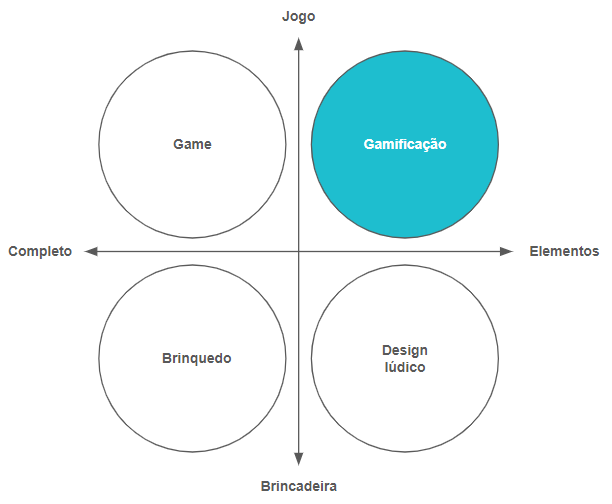
\includegraphics[width=0.5\textwidth]{figuras/Gamificação.png}
    \legend{Elaboração Própria}
\end{figure}


\section{Tabela}

\begin{table}[ht]
  \caption{Comparativo entre ferramentas similares}
  \label{Tab: Comparativo EA}
  \centering
  
  \begin{tabularx}{\textwidth}{p{4.4cm} ccccc}
    \hline
    \footnotesize\bfseries{Software} & \footnotesize\bfseries{Astronomia}   & \footnotesize\bfseries{Astronáutica}  & \footnotesize\bfseries{Mobile}  & \footnotesize\bfseries{Gamificação} & \footnotesize\bfseries{Português}\\
    \hline
    
        \footnotesize{Astronomia}              & x &   & x & x & x \\
        \footnotesize{Astronomy}               & x &   & x &   &   \\
        \footnotesize{Curso de Astronomia}     & x &   & x &   & x \\
        \footnotesize{ESApp}                   & x & x & x &   & x \\
        \footnotesize{Nasa}                    & x & x & x &   & x \\
        \footnotesize{Pockocmoc}               & x & x & x &   &   \\
        \footnotesize{Space Launch Now}        &   & x & x &   & x \\
        \footnotesize{Spacetoday}              & x & x &   &   & x \\
        \footnotesize{Stellarium}              & x &   & x &   & x \\
        \footnotesize{Space Learn}             & x & x & x & x & x \\ 
   
    \hline
  \end{tabularx}

  \legend{Elaboração Própria}
\end{table}

\section{Quadro}

\begin{quadro}[ht]
    \caption{Estrutura do GDD}
    \label{quad:gdd}
    \centering
    \begin{tabular}{|ll|}
        \cline{1-2}
        I.      & Resumo do Jogo            \\
        II.     & Descrição do Jogo         \\
        III.    & Informações Básica        \\
        IV.     & Planejamento Interno      \\
        V.      & Análises                  \\
        VI.     & Gameplay                  \\
        VII.    & Níveis                    \\
        VIII.   & Controle de versão        \\
        IX.     & Cronograma                \\
        \cline{1-2}
    \end{tabular}
    
    \legend{Elaboração Própria}
\end{quadro}

\vspace{2cm}

\section{Tabela grande}
\begin{table}[ht]
    \caption{Critérios da Técnica de Thomas Reeves}
    \label{Tab: CriterioThomas}
    \centering
    
    \begin{tabularx}{\textwidth}{m{.4cm} m{5cm} l}
        
        \hline
        \multicolumn{2}{c}{\footnotesize\bfseries{Critérios}} & \multicolumn{1}{c}{\footnotesize\bfseries{Conceitos}}\\
        \hline
        
        \multirow{14}{*}{\footnotesize\rotatebox{90}{Critérios Pedagógicos}}
        & \footnotesize{1. Epistemologia}                                 & \footnotesize{Objetivista              $\longleftrightarrow$ Construtivista}                  \\
        & \footnotesize{2. Filosofia Pedagógica}                          & \footnotesize{Instrutivista            $\longleftrightarrow$ Construtivista}                  \\
        & \footnotesize{3. Psicologia Subjacente}                         & \footnotesize{Comportamental           $\longleftrightarrow$ Cognitiva}                       \\
        & \footnotesize{4. Objetividade}                                  & \footnotesize{Precisamente Focalizado  $\longleftrightarrow$ N-Focalizado}                    \\
        & \footnotesize{5. Sequenciamento Instrucional}                   & \footnotesize{Reducionista             $\longleftrightarrow$ Construtivista}                  \\
        & \footnotesize{6. Validade Experimental}                         & \footnotesize{Abstrato                 $\longleftrightarrow$ Concreto}                        \\
        & \footnotesize{7. Papel Instrutor}                               & \footnotesize{Provedor de Materiais    $\longleftrightarrow$ Agente}                          \\
        & \footnotesize{8. Valoriazação do Erro}                          & \footnotesize{Aprendizado sem Erro     $\longleftrightarrow$ Aprendizado com a experiência}   \\
        & \footnotesize{9. Motivação}                                     & \footnotesize{Extrínseca               $\longleftrightarrow$ Intrínseca}                      \\
        & \footnotesize{10. Estruturação}                                 & \footnotesize{Alta                     $\longleftrightarrow$ Baixa}                           \\
        & \footnotesize{11. Diferenças individuais}                       & \footnotesize{Não existente            $\longleftrightarrow$ Multi-facetada}                  \\
        & \footnotesize{12. Controle do Aluno}                            & \footnotesize{Não existente            $\longleftrightarrow$ Irrestrito}                      \\
        & \footnotesize{13. Atividade do Usuário}                         & \footnotesize{Matemagênico             $\longleftrightarrow$ Generativo}                      \\
        & \footnotesize{14. Aprendizado Cooperativo}                      & \footnotesize{Não suportado            $\longleftrightarrow$ Integral}                        \\
    
        \hline
        
        \multirow{10}{*}{\footnotesize\rotatebox{90}{Critérios de Interface}}
        & \footnotesize{15. Facilidade de Uso}                            & \footnotesize{Difícil                  $\longleftrightarrow$ Fácil}                           \\
        & \footnotesize{16. Navegação}                                    & \footnotesize{Difícil                  $\longleftrightarrow$ Fácil}                           \\
        & \footnotesize{17. Carga Cognitiva}                              & \footnotesize{Não                      $\longleftrightarrow$ Gerenciável / Intuitiva}         \\
        & \footnotesize{18. Mapeamento}                                   & \footnotesize{Nenhum                   $\longleftrightarrow$ Poderoso}                        \\
        & \footnotesize{19. Design de Tela}                               & \footnotesize{Princípios violados      $\longleftrightarrow$ Princípios respeitados}          \\
        & \footnotesize{20. Simetria do Conhecimento}                     & \footnotesize{Incompatível             $\longleftrightarrow$ Compatível}                      \\
        & \footnotesize{21. Apresentação da Informação}                   & \footnotesize{Confusa                  $\longleftrightarrow$ Clara}                           \\
        & \footnotesize{22. Integração das Mídias}                        & \footnotesize{Não Coordenada           $\longleftrightarrow$ Coordenada}                      \\
        & \footnotesize{23. Estética}                                     & \footnotesize{Desagradável             $\longleftrightarrow$ Agradável}                       \\
        & \footnotesize{24. Funcionalidade Geral}                         & \footnotesize{Não funciona             $\longleftrightarrow$ Altamente funcional}             \\
        
        \hline
    \end{tabularx}
    
    \legend{Adaptado de \citeonline{Cybis:00}}
\end{table}

\clearpage

% https://www.seer.ufrgs.br/index.php/renote/article/view/53496/33013
% \footnotemark
% \footnotetext {Disponível em: <>. Acesso em: xx ______ xxxx.}
